%TODO Make sure to link help page for scipy.special.erfc
%TODO Change instrumental instructions to
%	- Remove guidance about changing PMT voltage (keep at high value for all experimentes)
%	- Add in comment to check baseline zero level before beginning

\maketitle% this prints the handout title, author, and date

\begin{abstract}
\noindent
The objective of this lab is to determine the rate constant and collision diameter of a diffusion-controlled reaction (photoexcited anthracene with carbon tetrabromide, \ch{CBr4}) using the technique of fluorescence quenching.\thanks{Transcribed (with corrections) from \textcite{halpern97}.}
\end{abstract}

%\printclassoptions


\section{Introduction} % (fold)
\label{sec:intro}

In this experiment, you will study a very fast bimolecular reaction between two different species in solution. 
Let us assume that the reactants, \ch{A} and \ch{B}, which are electrically neutral, undergo independent, random motion in solution. 
There is a certain probability that \ch{A} and \ch{B} will encounter each other at some close distance, \(R\), where \(R\) is approximately equal to the sum of their molecular radii. 
This arrangement is called an \emph{encounter complex}. 
Because there is a tendency for the solutes \ch{A} and \ch{B} to maintain constant random motion, it is inevitable that, once
loosely held in this complex, they will subsequently separate from each other unless a chemical
reaction (or other definitive process) first links them together or causes them to react. 
Since this random motion takes place in a ``bath'' of solvent molecules (assumed to be unreactive with respect
to \ch{A} and \ch{B}), the separation of the \ch{A-B} encounter complex will be impeded by the neighboring
solvent molecules. 
This artificial holding-together of the two molecules is called the \emph{cage effect}.
The important point is that there is a kinetic competition between a net (thus measurable) reaction
between \ch{A} and \ch{B} via the collision complex, and the release of \ch{A} and \ch{B} from the solvent cage back
into the solvent medium where no reaction occurs. 
We can represent these processes by the following kinetic scheme:
\begin{align}
\begin{split}
	\ch{A_{solv} + B_{solv} <=>[$k\sb{1}$][$k\sb{-1}$] (A-B)_{solv}} \, , \\
	\ch{(A-B)_{solv} ->[$k\sb{2}$] \text{product(s)}} \, ,
\end{split}
\label{eq:rxn_scheme}
\end{align}
where \ch{A_{solv}} and \ch{B_{solv}} represent the solvated \ch{A} and \ch{B} molecules and \ch{(A-B)_{solv}} is the solvated encounter complex. 
The rate constants for these elementary steps are denoted as \( k_1 \), for the bimolecular formation of the encounter complex (or diffusion into the solvent cage); \( k_{-1} \), for the unimolecular dissociation of the complex (or diffusion out of the solvent cage); and \( k_2 \) for the ``unimolecular'' reaction between \ch{A} and \ch{B} in the complex to form the product(s). 

Because we assume that the encounter complex undergoes rapid deactivation, either by
dissociation or via reaction, we can employ the steady-state approximation, according to which
the net formation rate of \ch{(A-B)_{solv}} is zero. Thus
\[
	\dv{\ch{[A-B]}}{t} = k_1 \ch{[A][B]} - (k_{-1} + k_2)\ch{[A-B]} = 0 \, ,
\]
and we can approximate the steady-state concentration of the encounter complex as 
\[
	\ch{[A-B]} \simeq \frac{k_1\ch{[A][B]}}{k_{-1}+k_2} \, .
\]

Now, if we further assume that the reaction rate is given by the slow step, i.e., \( k_2 \)\ch{[A-B]}, we can express that rate as
\[
	\text{Rate} \simeq k_2 \ch{[A-B]} = \frac{k_1 k_2}{k_{-1} + k_2} \ch{[A][B]} = k_\mtext{obs}\ch{[A][B]} \qquad \si{ \per \s} \, .
\]
For convenience, we define the second-order rate coefficient, \( k_\textup{obs} \), as 
\begin{equation}
	k_\textup{obs} = \frac{k_1 k_2}{k_{-1} + k_2} \, .
	\label{eq:k_obs}
\end{equation}

This analysis leads to two limiting cases with respect to \( k_\textup{obs} \): 
\begin{enumerate}
	\item the reaction between \ch{A} and \ch{B} is very slow compared with their departure (and separation) from the solvent cage, i.e., \( k_{-1} \gg k_2 \); and 
	\item the \ch{A-B} reaction is much faster than their separation, or \( k_2 \gg k_{-1} \). 
\end{enumerate}
The first case describes a reaction that is under \emph{chemical} control, with \( k_\textup{obs} \simeq k_1 k_2 / k_{-1} \), and the second pertains to a \emph{diffusion-controlled} reaction for which \( k_\textup{obs} \simeq k_1 \). 
The latter situation is considered in this experiment. More details of the reaction, which involves fluorescence quenching, will be described after a discussion of the relevant theoretical ideas.\sidenote{
	Note from the discussion that, when the actual reaction occurs fast enough within the solvent cage (\emph{i.e.} when \( k_2 \) is very large compared to \( k_{-1} \)), \( k_\textup{obs} \approx k_1 \). 
	From the definition contained in \cref{eq:rxn_scheme}, \( k_1 \) is the rate constant for the diffusion of the reactants through the solvent. 
	Therefore, this condition means that this diffusion step is actually rate limiting for the overall reaction. 
	Once the reactants are close enough to one another, they will react almost instantaneously. 
	This also implies that such a reaction would have essentially no activation barrier.
} 
% section intro (end)

\section{Diffusional Mass Transport} % (fold)
\label{sec:mass_trans}
The basic issue in a diffusion-controlled reaction concerns the dynamics of mass transport in the condensed phase. 
The fundamental equations describing mass transport are embodied by Fick's laws of diffusion. 
Fick's first law says that the number of molecules, \( \dd{n} \), diffusing through a unit area, \( A \), per unit time, \( \dd{t} \), in the \emph{x} direction (i.e., the flux, \( J_x \)) is proportional to the concentration gradient at that point, i.e.,
\begin{equation}
	J_x \equiv \frac{1}{A}\dv{n}{t} = -D \dv{C}{x} \, ,
	\label{eq:fickA}
\end{equation}
where the proportionality constant \( D \) is called the \emph{diffusion coefficient}. 
The units of \( D \) are \si{\cm\squared \per \s}. 
The minus sign in \cref{eq:fickA} indicates that transport goes against the concentration gradient
(i.e., from high to low concentration values).

Fick's second law states that the change in the concentration of molecules, \( \dd{C} \), diffusing
across an infinitesimally thin plane per unit time, \( \dd{t} \), is proportional to the gradient of the flux:
\begin{equation}
	\br{\dv{C}{t}}_x = - \br{\dv{J_x}{x}}_t \, .
\end{equation}
Again, the minus sign ensures that the concentration increases in time in response to a flux that decreases with increasing \( x \).
If we assume \( D \) to be independent of \( x \), we may substitute the expression for \( J_x \) from Fick's first law into the second to give
\begin{equation}
	\br{\dv{C}{t}}_x = D \br{\dv[2]{C}{x}}_t \, .
	\label{eq:fickBa}
\end{equation}
Because we are concerned with a three-dimensional and isotropic space, i.e., equal forces in all directions, we can write Fick's second law in a more general form as 
\begin{equation}
	\br{\dv{C}{t}}_{x, y, z} = D \br{\laplacian{C}}_t \, ,
	\label{eq:fickBb}
\end{equation}
where \( \laplacian{} \) is the Laplacian operator \( \pdv*[2]{x} + \pdv*[2]{y} + \pdv*[2]{z} \).

The solution of Fick's second law is an equation that expresses concentration as a function of \emph{space} (i.e., distance), \( r \), and \emph{time}, \( t \). 
We are interested in solving \cref{eq:fickBb} with the boundary conditions 
\begin{align*}
	C(r, 0) 		&= C_0 \, , \\
	C(\infty, t) 	&= C_0 \, , \\
	C(r=R, t) 	&= 0 \, ,
\end{align*}
where \( r = \sqrt{x^2 + y^2 + z^2} \), and \( C_0 \) denotes the \emph{bulk} concentration. 

The first boundary condition states that, initially, the bulk concentration prevails throughout the system; the second says that, even after the reaction starts \( (t > 0) \), the concentration very far away from the reactant, i.e., the bulk concentration, \( C_0 \), is constant; and the third indicates that the reactant concentration is zero at a distance equal to the sum of the reactant collision radii. 
Note that the diffusion coefficient, \( D \), contained in \cref{eq:fickA,eq:fickBa,eq:fickBb} is the sum of the individual diffusion coefficients of the reactants, \( D_{\ch{A}} + D_{\ch{B}} \). 
This expression essentially allows the motion of one of the reactants to be considered relative to the other. 

The solution of Fick's second law for this set of boundary conditions (first rendered by Smoluchowski in 1917) yields, for the space-time dependence of \emph{C},
\begin{equation}
	C(r, t) = C_0 \br{ 1 - \frac{R}{r} \erfc\br{ \frac{r-R}{2 \sqrt{D t} }}} \, , 
\end{equation}
in which \( \erfc(x) \) is the \emph{complementary error function}, \( 1 - \erf(x) \), defined as
\[
	\erfc(x) \equiv 1 - \frac{2}{\sqrt{\pi}}\int_0^x \exp\br{ -y^2 } \dd{y} \, .
\]
The time dependence of the reactant at the reaction boundary \( r = R \) becomes expressible in terms of the flux of reactant, \( J_R \), or its rate of transport across a hypothetical spherical surface with radius \( R \). 
Thus
\begin{equation}
	J_R = \frac{4\pi R D N_\mtext{A} C_0}{1000} \br{ 1 + \frac{R}{\sqrt{\pi D t}}} \qquad \si{molecules \per \s} \, ,
	\label{eq:rxnbound}
\end{equation}
where \( N_\mtext{A} \) is Avogadro's number. 
The units shown (and factor of 1000) pertain if \( C_0 \) is expressed in molarity (\si{\mol\per\liter}) and \( R \) and \( D \) are expressed in \si{\cm} and \si{\cm\squared \per \s}, respectively.\sidenote{
To convert from \si{molecules} to \si{\Molar}, we need to acount for the number of particles in a \si{mole} (Avogadro's number) and convert from our molecular length units (\si{\cm}) to proper volume units. It's useful to know that \( \SI{1}{\L} =\SI{1}{\dm\cubed} \).}
\Cref{eq:rxnbound} indicates that the flux (molecules per unit area per second) is actually time-dependent. 
This time dependence comes from \( R/\sqrt{\pi D t} \), which is sometimes referred to as the \emph{transient term}. 
Physically, the transient term accounts for the fact that initially nearby reactant molecules do not have to diffuse through the bulk medium in order to react. 
After a short time, however, these nearby reactant molecules are depleted, and the flux approaches a constant, or steady-state, value, \( 4\pi R D N_\mtext{A} C_0 / 1000 \). 
This can be seen mathematically in that time is represented in \cref{eq:rxnbound} as \( \sqrt{t} \). 

Because \( J_R \) represents the rate of passage of one of the reactants (having a bulk concentration \( C_0 \) in \si{\Molar}) through a spherical reaction surface with the other reactant at the center, the rate of the reaction represented by \cref{eq:rxn_scheme} is merely \( J_R \) itself. 
Hence, the bimolecular, diffusion-controlled rate constant \( k_1 \) is \( J_R/C_0 \),
\begin{equation}
	k_1 = \frac{4 \pi R D N_\mtext{A}}{1000} \br{ 1 + \frac{R}{\sqrt{\pi D t}}} \qquad \si{\per\Molar \per\s} \, .
	\label{eq:rateconst1}
\end{equation} 
This rate constant is not a true \emph{constant}, however, because of the transient term. 
However, as \( t \) becomes large enough,
\begin{equation}
	\lim_{t \to \infty} k_1 = \frac{4 \pi R D N_\mtext{A}}{1000} \qquad \si{\per\Molar \per\s} \, ,
	\label{eq:rateconst2}
\end{equation}
and \cref{eq:rateconst2} can be used to determine the diffusion-controlled rate constant if the mutual diffusion constant \( (D_\mtext{A} + D_\mtext{B}) \) and collision radii \( (R_\mtext{A} + R_\mtext{B}) \) are known.\sidenote[][-13\baselineskip]{
	An important consideration in \cref{eq:rateconst1,eq:rateconst2} is the time dependence of \( k_1 \). 
	We do not typically think of rate constants as changing in time, but \cref{eq:rateconst1} contains a \emph{transient term}, \( R/\sqrt{\pi D t} \). 
	Remember that the diffusion, or movement of the molecules through the solvent, is the slow step of this reaction and is rate determining. 
	However, at the very beginning there will be some fraction of molecules that are already close enough together to react without needing to diffuse. 
	Therefore, the apparent rate of the reaction will be faster initially. 
	As these pairs react, this population is depleted, leaving behind reactants that are farther apart and thus need to undergo diffusion. 
	Thus, the transient term dies out and the reaction finally reaches a purely diffusion controlled regime, described by the rate constant in \cref{eq:rateconst2}.
	}
We emphasize again that the units of \( k_1 \) presented above are \si{\per\Molar \per \s}, if \( R \) and \( D \) are expressed in \si{\cm} and \si{\cm\squared \per \s}, respectively. 

Often, however, \( R \) and \( D \) are not known, and an indirect method is used to estimate \( k_1 \). 
This approach, developed by Einstein using Stokes's law, allows the diffusion coefficient to be expressed in terms of a bulk property, the solvent viscosity, \( \eta \). Thus
\begin{equation}
	k \simeq \frac{8 \overline{R} T}{3 \eta} \qquad \si{\per\Molar \per \s} \, ,
	\label{eq:rateapprox}
\end{equation}
where \( \overline{R} = k_\mtext{B} N_\mtext{A} \) is the ideal gas constant.%
\sidenote[][-6\baselineskip]{
	Note the distinction between \( \overline{R} \) and \( R \). 
	\( \overline{R} \) appears \emph{only} in this equation and refers to the gas constant. 
	Everywhere else, \( R \) is the summed ``collision radii'' of the interacting species. 
	It is this collision radius that we are trying to find in this experiment, along with the rate constant \( k_1 \). 
	Also, keep in mind that \cref{eq:rateapprox} represents and \emph{alternative} method for estimating the diffusion rate constant, \( k_1 \), based on bulk parameters of the solvent, rather than detailed knowledge of the molecular parameters \( R \) and \( D \).
	}
\Cref{eq:rateapprox}, which is often referred to as the Stokes-Einstein-Smoluchowski (SES) equation, holds when the reactants \ch{A} and \ch{B} are different and their sizes are larger than that of the solvent molecules. 
The indicated units are obtained if \( \overline{R} \) and \( \eta \) are expressed in SI units, such that \( \overline{R} = \SI{8.314e3}{\L \Pa \per \mol \per \K} \) and \( \eta \) is in \si[inter-unit-product=\ensuremath{{}\!\cdot\!{}}]{\Pa \s}.
% section mass_trans (end)

\section{Fluorescence Quenching} % (fold)
\label{sec:fl_quenching}

The reaction studied in this experiment takes place between an electronically excited molecule and a quencher, a species that removes the electronic excitation. 
The advantages of using an electronically excited molecule as one of the reactants are: 
1) the reaction takes place only when the system is exposed to light; 
2) the concentration of electronically excited molecules can be readily followed fluorometrically (via fluorescence detection); and 
3) the reaction itself is intrinsically fast---it has no activation energy \emph{per se}, and is limited by the encounter between the excited molecule and the quencher. 
Many experiments utilize luminescence quenching as a ``kinetic'' technique. 
The overall reaction describing fluorescence quenching can be represented as
\[
	\ch{A\!^* + Q -> product(s)}
\]
where \ch{A\!^*} represents the electronically excited (fluorescent) state of a molecule (e.g., anthracene in this experiment), \ch{Q} denotes the quencher (e.g., \ch{CBr4}) that ``extinguishes'' the \ch{A\!^*} fluorescence, and ``product(s)'' indicates the species into which the fluorescent molecule is eventually transformed. 
This de-excitation process may occur through a charge-transfer intermediate (\ch{A^{+}—Q-}) in which electronic charge is transferred to the quencher molecule from the excited-state species.
For the system encountered in this experiment, electron transfer from \ch{A\!^*} to the quencher occurs very rapidly. 
In general, it is possible that the consequence of fluorescence quenching is the return of \ch{A} to its electronic ground state without any change in structure, i.e., \ch{A + Q}.

In the case of \ch{CBr4}, the quenching mechanism involves the electron transfer from the excited state, \ch{A\!^*}, to \ch{CBr4}, which is more electronegative than \ch{A\!^*}. 
A reverse electron transfer then restores the two molecules to their neutral species, \ch{A} being in the ground state. 

The bimolecular quenching reaction shown above, however, competes with the intrinsic first-order fluorescence decay of \ch{A\!^*} and thus reduces the probability that the \ch{A\!^*} species will emit a photon. A more complete scheme is thus
\begin{align*}
	\ch{A 			&	&	->[\hphantom{\(k\sb{r}\)}]&	&	&	A\!^*&														&"(photoexcitation)"} \\
	\ch{A\!^* 		&	&	->[\(k\sb{\mtext{r}}\)]&	&	&						A + \(h\nu\sb{\mtext{f}}\)&							&"(fluorescence)"} \\
	\ch{A\!^* 		&	&	->[\(k\sb{\mtext{nr}}\)]&	&	&						A&															&"(nonradiative~decay)"} \\
	\ch{A\!^* + Q	&	&	->[\(k\sb{\mtext{q}}\)]&	&	&						"electron~transfer" + "\ldots"&	&"(quenching)"}
\end{align*}

If a solution containing \ch{A} and \ch{Q} is irradiated with a \emph{steady-state} light source (at a wavelength where \ch{A} absorbs), a very small time-independent concentration of \ch{A\!^*} is produced. 
The probability that \ch{A\!^*} will fluoresce, \( P_\mtext{f} \), is the ratio of the fluorescence (or radiative) rate constant to the sum of all the rate constants that deplete \ch{A\!^*}, namely,
\begin{equation}
	P_\mtext{f} = \frac{k_\mtext{r}}{k_\mtext{r} + k_\mtext{nr} + k_\mtext{q} \ch{[Q]}}
	\label{eq:prob_fluor}
\end{equation}
where \( k_\mtext{r} \), \( k_\mtext{nr} \), and \( k_\mtext{q} \)\ch{[Q]} are, respectively, the radiative, nonradiative, and (pseudo-first-order) quenching rate constants, 
Since \( \ch{[Q]} \gg \ch{[A\!^*\,]}\), the diffusion-controlled bimolecular quenching step becomes pseudo-first-order. 
If the amount of light absorbed by \ch{A} is unaffected by \ch{[Q]}, the fluorescence \emph{intensity}, \( I \), measured by the detector (i.e., the instrument response) is proportional to \( P_\mtext{f} \). 
In the absence of quencher, \( I = I_0 = k_\mtext{r} / (k_\mtext{r} + k_\mtext{nr}) \), and the ratio of fluorescence intensities of unquenched to quenched samples of \ch{A} becomes 
\begin{equation}
	\frac{I_0}{I} = 1 + \frac{k_\mtext{q} \ch{[Q]}}{k_\mtext{r} + k_\mtext{nr}} \, .
	\label{eq:quench_ratio}
\end{equation}
Identifying \( 1/(k_\mtext{r} + k_\mtext{nr}) \) as the reciprocal of the \emph{fluorescence lifetime} of \ch{A\!^*} in the absence of quencher \( (\tau_0) \), we can write \cref{eq:quench_ratio} as 
\begin{equation}
	\frac{I_0}{I} - 1 = k_\mtext{q} \tau_0 \ch{[Q]} \, .
	\label{eq:sv_rel}
\end{equation}

\Cref{eq:sv_rel} is known as the steady-state Stern-Volmer (S-V) relation as applied to fluorescence quenching. 
It predicts that a plot of \( I_0/I - 1 \) vs. \ch{[Q]} should be linear, having an intercept of zero and a slope equal to \( k_\mtext{q} \tau_0 \). 
The latter is called the Stern-Volmer constant, \( K_\mtext{SV} \) (units of \si{\per\Molar}). 
If fluorescence quenching is diffusion-controlled (which is the case in the anthracene/\ch{CBr4} system), \( k_\mtext{q} \) can be identified with \( k_1 \) (see \cref{eq:rxn_scheme,%
eq:k_obs,eq:rateconst1,eq:rateconst2,eq:rateapprox}).\sidenote[][-9\baselineskip]{
	The first Stern-Volmer Equation \cref{eq:sv_rel} is generally applicable because it makes no assumptions about the quenching rate constant \( k_\mtext{q} \). 
	Since we are dealing with a diffusion-controlled reaction, we can identify \( k_\mtext{q} \) with the diffusion-controlled rate constant, \( k_1 \), from \cref{eq:rateconst1,eq:rateconst2,eq:rateapprox}. 
	It should therefore be straightforward to measure the fluorescence emission of some analyte \ch{A} as we change the concentration of the quencher \ch{Q}, and fit the data to \cref{eq:sv_rel} to obtain a value for \( k_1 \). 
	However, this still leaves us with a question: Does the \( k_1 \) obtained in this manner correspond to \cref{eq:rateconst1}, \cref{eq:rateconst2}, or \cref{eq:rateapprox}?

	\Cref{eq:rateconst2,eq:rateapprox} do not depend on the time, \( t \), and therefore correspond to the steady-steady state regime where the reaction is fully diffusion-controlled. 
	When combined with \cref{eq:sv_rel}, they describe a linear Stern-Volmer plot in which the slope is equal to \( k_1 \tau_0 \).

	\Cref{eq:rateconst1}, however, includes a time dependence of \( k_1 \). 
	The expression cannot simply be inserted into \cref{eq:sv_rel} without carrying this time dependence along with it. 
	Since we are not measuring the quenching as a function of time, this doesn’t help us. 
	Instead, the Stern-Volmer Equation can be re-derived, taking into account the transient term, to obtain \cref{eq:sv_step_rel}.
}

In the absence of the transient effect, which is a type of ``static'' quenching in that some \ch{A\!^*} molecules are quenched by nearby \ch{Q} molecules that do not have to undergo transport fully through the solvent medium in order to approach \ch{A\!^*} within a distance \( R \), the S-V plot should be linear, and independent knowledge of \( \tau_0 \) allows us to determine \( k_\mtext{q} \). 
Alternatively, if the process is known to be diffusion-controlled, and if \( k_1 \) is determined from the SES (or some other) equation (e.g., \cref{eq:rateconst2}), the fluorescence lifetime of \ch{A\!^*} can be estimated from the measured \( K_\mtext{SV} \) value. 
This is a case in which a dynamic property (a rate constant) can be obtained from a static experiment (\( I_0/I \) measurements). 


The S-V relation can be expressed in terms of the diffusion-controlled rate constant that contains the transient term, e.g., \cref{eq:rateconst1}. 
The time dependence was treated by \textcite{ware66}, who applied \cref{eq:rateconst1} to the condition pertinent to this experiment, namely, that the system is considered to be suddenly exposed to a steady-state excitation source, called a step function (see \cref{fig:step_func} and Further Readings). %
\begin{marginfigure}
	\centering
	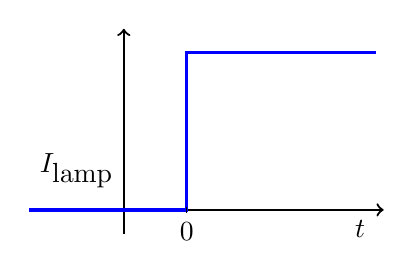
\begin{tikzpicture}
			\draw[->, thick] (-1.2, 0) -- (2.2,0) node[below] {$t$} -- (2.5,0);
			\draw[->, thick] (-0.8, -0.3) -- (-0.8,0.5) node[left] {$I_\textup{lamp}$} -- (-0.8,2.3);
		
			\draw[very thick, blue]
				plot[const plot] coordinates {(-2,0) (0,2) (2.4,2)};
			\draw (0,1pt) -- (0,-1pt) node[below] {$0$};
	\end{tikzpicture}
	\caption{A ``step excitation''\\ function (known in mathematics as a ``Heaviside function''). At time \( {t = 0} \), absorbing radiation is suddenly ``switched on.''}
	\label{fig:step_func}
\end{marginfigure}%
In this case, the S-V equation becomes more complicated:
\begin{equation}
	\frac{I_0}{I} = \frac{1 + (4 \pi R D N_\mtext{A} / 1000) \ch{[Q]} \tau_0}{Y} \, ,
	\label{eq:sv_step_rel}
\end{equation}
where
\begin{equation}
	Y = 1 - \frac{b \sqrt{\pi}}{\sqrt{a}} \exp\br{\br{ \frac{b^2}{a} }} \erfc\br{ \frac{b}{\sqrt{a}} } \, ,
	\label{eq:sv_y}
\end{equation}
in which 
\begin{align*}
	a &= \frac{1}{\tau_0} + \frac{4 \pi R D N_\mtext{A}}{1000} \ch{[Q]} \qquad \si{\per\s} \, ,\\
	b &= \frac{4 \sqrt{\pi D} R^2 N_\mtext{A}}{1000} \ch{[Q]} \qquad \si{\sqrt{1\per\s}}\, .
\end{align*}
If \( Y = 1 \), \cref{eq:sv_step_rel} reduces to \cref{eq:sv_rel},\sidenote{
	\Cref{eq:sv_step_rel} describes a curved line due to the transient effects that take place very soon after the light source is switched on. 
	However, this may cause some confusion, because our Stern-Volmer plots do not involve a time variable. How can the transient effects account for this curvature, if there is no explicit time dependence?
	We touched on the answer to this before, but it is worth emphasizing again. 
	The transient term arises because when the light source is first switched on there are some \ch{A/Q} pairs that are close enough to react without diffusing very far. 
	Since the overall rate of the reaction can be thought of as an average of the rates for each individual molecular collision, the faster reactions between these pairs will skew the average towards faster rates. 
	This statistical effect will be much more significant when there is a very high concentration of one or both components, and almost negligible when the concentrations are very low. 
	Since the slope of the Stern-Volmer plot is proportional to the rate constant, \( k_1 \), this means that the slope will be large (faster rates) at high quencher concentrations, \ch{[Q]}, and small (slower rates) at low \ch{[Q]}. We will explore how these conditions relate to the other Stern-Volmer equation (\cref{eq:sv_rel}) in the Data Analysis section below.
	} 
in which case \( k_\mtext{q} = k_1 \) from \cref{eq:rateconst2}.\sidenote{Verify this for yourself!}

The Stern-Volmer plot based on \cref{eq:sv_step_rel} should be curved upward. 
If the mutual diffusion coefficient of the reacting pair is known, the S-V plot of experimental data can be fit using \cref{eq:sv_step_rel} with \( R \) used as a ``fitting'' parameter. 
For a satisfactory match between experiment and theory, however, the value of \( R \) must be physically reasonable. 
That is, \( R \) should be approximately equal to the sum of the molecular diameters of \ch{A} (actually \ch{A\!^*\,}) and \ch{Q}.


% section fl_quenching (end)

\pagebreak

\section{Safety Precautions} %(fold)
\label{sec:safety}

\begin{itemize}
	\item Always wear safety glasses or goggles; these glasses should block ultraviolet light. 
	Ordinary plastic safety goggles or glasses may not be effective in absorbing all the ultraviolet radiation. 
	Check with your instructor.
	\item Do not allow solid anthracene to come in contact with the skin. 
	Wear gloves when handling anthracence and \ch{CBr4}.
	\item Ozone is sometimes produced by ultraviolet light sources. 
	If you detect this gas, which has a sharp, slightly acrid odor, notify your instructor and immediately shut off the source.
	Increase ventilation, and leave the room immediately.
	\item The compressed-gas cylinder used in deaerating should be securely strapped to a firm support.
	The delivery pressure should never exceed a few (e.g., 5) \si{\psig}.
	\item The experiment should be performed in an open, well-ventilated laboratory.
\end{itemize}
% section safety (end)


\section{Procedure} % (fold)
\label{sec:procedure}

\subsection{Required Equipment} % (fold)
\label{sub:required_equipment}

\begin{itemize}
	\item (10) \SI{10}{\mL} volumetric flasks
	\item (1) \SI{10}{\ml} graduated pipet
	\item (1) fluorescence cell
	\item dry nitrogen gas cylinder
\end{itemize}

% subsection required_equipment (end)


\begin{enumerate}
	\item Using freshly sublimed or purified anthracene and \ch{CBr4}, prepare \SI{250}{\mL} of \SI{\sim1.00E-4}{\Molar} solution of anthracene (\ch{AN}) in spectrometric (or fluorometric) quality \emph{n-}hexane. 
	Using this solution as ``solvent,'' prepare \SI{25}{\mL} of \SI{\sim1.50E-2}{\Molar} ``stock'' solution of \ch{CBr4}.
	\item Prepare at least eight dilutions of the \ch{AN}/\ch{CBr4} stock solution using the \ch{AN} solution as solvent.
	The most dilute should be \SI{5}{\percent}, and the rest should be nearly evenly spaced up to the stock-solution value. 
	A volume of \SI{10}{\mL} of each solution is appropriate. 
	Include \SIlist{0;100}{\percent} samples for uniformity. 
	Label these samples.
	\item Starting with the \SI{0}{\percent} sample (\ch{AN} only), introduce the solution into a fluorescence cell and deaerate with dry \ch{N2} for about \SI{2}{\min}. 
	Avoid using an excessive flow rate that will cause the solution to splatter from the cell or to otherwise result in undue solvent evaporation. 
	Promptly stopper the cell.
	\item Record the full fluorescence spectrum using the instrumental conditions previously outlined by the instructor.\sidenote{
\begin{tabular}{lr}
  \toprule
  Parameter & Value\\
  \midrule
  \( \lambda_\mtext{exc} \) & \SI{283}{\nm}\\
  \( \lambda_\mtext{det} \) & \SIrange{350}{550}{\nm}\\
  Scan speed & \SI{300}{\nm\per\min}\\
  Slit width & \SI{2.5}{\nm}\\
  \bottomrule
\end{tabular}}
	Make sure the spectrum record is labeled.
	\item Using exactly the same settings as in step 4, measure the  fluorescence intensity of the most dilute and subsequently more concentrated \ch{AN}/\ch{CBr4} solutions. 
	You must deaerate each sample in a consistent procedure (i.e., identical bubbling time). 
	If you have any doubt as to the steadiness of the exciting source, switch back to the \ch{AN} sample and compare its maximum intensity with that of the first sample run.
	\item As you examine increasingly more concentrated samples, the fluorescence intensity will diminish to the point that you may need to increase the instrument gain (i.e., signal amplification) to ensure maximal reading sensitivity. 
	Establish the background, or ``dark check,'' when the instrument sensitivity is changed.
  This gain should result in a linear increase in signal, but you should take spectra of one concentration twice (once at each gain level) to provide a way to scale your spectra. 
	\item Keep in mind the following procedural points: 
	\begin{enumerate}
		\item The temperature of the sample should be held constant within \SIrange{0.5}{1.0}{\celsius}; 
		\item the exposure times of all of the samples (especially those rich in \ch{CBr4}) to the excitation source (and even room light) should be minimized; and 
		\item samples should be stored in the dark until they are used.
	\end{enumerate}
\end{enumerate}

% section procedure (end)

\section{Data Analysis} % (fold)
\label{sec:data_analysis}
\begin{enumerate}
	\item Tabulate your data as \( I \) (the anthracene fluorescence at \num{398} or \SI{399}{\nm}) and \ch{[Q]} (the \ch{CBr4} concentration, in \si{\Molar}).\marginnote{This is a good place to practice with the Pandas library. 
  All of your spectra should use the same wavelength range, so you can import the CSV data and set the index column to the wavelength.
  You can then find the wavelength for the maximum fluorescence and grab the intensity at that wavelength for each sample.}
	\item Plot a graph of  \( I_0/I \)  vs. \ch{[Q]}. 
	Note that \( I_0 \) is simply the value of the unquenched fluorescence peak (when \( \ch{[Q]} = 0 \)). 
	This is your experimental quenching curve or Stern-Volmer plot, and we will now see how it corresponds to the two limits of the quenching model (with and without the transient term), as well as the SES equation.
	\item Begin by considering the Stokes-Einstein-Smoluchowski (SES) equation, \cref{eq:rateapprox}. 
	Use the gas constant, \( \overline{R} \), the temperature (assume \SI{25}{\celsius} and the viscosity of \emph{n-}hexane to calculate \( k_1 \). 
	Use the proper units as described in the manual. 
  Once you have \( k_1 \), insert it into \cref{eq:rateconst2} to calculate the collision radius \( R \) (don’t mix up \( \overline{R} \) and \( R \)).\sidenote[][-5\baselineskip]{
		To do this, you’ll need to calculate the diffusion coefficient, \( D \), for \emph{n-}hexane from the \( D \) known for \emph{n-}heptane. 
		\textcite{dymond94} gives values for the viscosity of various \emph{n}-alkanes. 
		\textcite{ware66} reported a value of \( D = \SI{4.35e-5}{\cm\squared \per \s} \) in \emph{n}-heptane at \SI{25}{\celsius}. 
		To obtain \( D \) for \emph{n}-hexane at some other temperature, assume that \( D \) is proportional to \( T/\eta \). 
		They also reported a value of \( \tau_0 = \SI{5.52e-9}{\s} \). You can assume this to be temperature independent.
	} 
	What is the collision radius calculated this way (including the unit)?\sidenote{%
	\textbf{Keep track of your units, especially \emph{moles} vs. \emph{molecules}.}}
	\item Using the \( k_1 \) you just calculated from the SES equation, superimpose the straight line obtained from \cref{eq:sv_rel} onto your Stern-Volmer plot. You’ll need the lifetime, \( \tau_0 \).\sidenote{
  To do this, you'll need to generate a set of \(x\)-values for your function, then apply your function to those values. 
  The help page for \( \erfc(x) \) linked above shows how to do this for that particular function. }
	Describe the relationship between this line and the experimental data points, if any.
	\item Now we will consider the Stern-Volmer plot obtained when we ignore the transient term. 
	Remember that this condition holds at low concentrations. 
	Therefore we will be looking for the tangent to the experimental curve near the \emph{y}-axis. 
	Take a few of the experimental data points close to \( \ch{[Q]} = 0 \), fit a trendline to them, and show the equation. 
	The points you include for this should all be nearly in a straight line. 
	If you take too many, they will begin to show the curvature and your slope will be incorrect. 
	From the slope of this tangent line, calculate an alternate value for \( k_1 \). 
	You’ll need the lifetime from the manual again. 
	From that value of \( k_1 \), calculate another value for the collision radius, \( R \), using \cref{eq:rateconst2}. How do these values of \( k_1 \) and \( R \) compare to the values calculated from the SES equation in step 3?
	\item Now we can examine the entire data set, which includes effects due to the transient-term, in order to extract a third value of \( R \) directly. 
	We will do this by fitting our data to \cref{eq:sv_step_rel} using a ``nonlinear regression analysis'' with \( R \) as the only parameter.%
	\sidenote{%
    To perform this step with Python, you will need to use the SciPy library. 
		Instructions and an example can be found in the SciPy Documentation under \href{https://docs.scipy.org/doc/scipy/reference/generated/scipy.optimize.curve_fit.html}{scipy.optimize.curve\_fit}. 
	} 
	Just make sure you realize that the parameter \( R \) enters into \cref{eq:sv_step_rel} directly in the numerator, as well as through the denominator \( Y \) due to the \( R \) dependence of \( a \) and \( b \). 
	Thus, you need to make sure that all of these parts of the equation refer to the same variable for \( R \) so that it is varied consistently throughout. 
	Make sure that you use \( \erfc() \) and not \( \erf() \). 
	You can start with a guess of \SI{10}{\angstrom} for the radius \( R \) and have \Verb{curve_fit()} solve for the best fit of your line. 
  Superimpose the theoretical curve corresponding to this \( R \) value onto your data points.
\end{enumerate}
% section data_analysis (end)

\section{Questions and Further Thoughts} % (fold)
\label{sec:questions_and_further_thoughts}

\begin{enumerate}
	\item Why is the anthracene fluorescence quenching diffusion-controlled as opposed to chemical-controlled? 
	I.e., justify why the reaction between \ch{AN^*} and \ch{CBr4} is very fast.
	\item What experiment(s) could you perform to determine whether a stable photoproduct is formed as a result of the fluorescence quenching?
	\item What could you do to obtain supporting evidence for the existence of a charge-transfer (or ion-pair) intermediate, e.g.,
	\[
		\ch{AN^* + CBr4 -> \big(AN^+\big)\big(CBr4^-\big) -> AN + CBr4}
	\]
	in the quenching process?
	\item Verify that if \( Y = 1 \) in \cref{eq:sv_step_rel}, \( k_\mtext{q} \rightarrow k_1 \) (see \cref{eq:sv_rel,eq:rateconst2}).
	\item One of the undesirable complications associated with this type of experiment is the potential presence of \emph{ground-state} complexes between \ch{AN} and \ch{CBr4}. 
	If such a complex competes for light absorption with uncomplexed, free anthracene, it can cause a decrease in fluorescence intensity without the existence of diffusion between \ch{AN^*} and \ch{CBr4}. 
	This is sometimes called \emph{static quenching}. 
	For this reason, it is desirable to work with quencher concentrations as low as possible. 
	What experiment could you do to obtain evidence of a ground-state complex? 
	How could you determine the equilibrium constant of such a complex?
	\item What effect would a polar solvent, e.g., acetonitrile (\ch{CH3CN}), have on the ground- and excited-state interactions between \ch{AN} and \ch{CBr4}?
	\item If you wanted to do a fluorescence quenching experiment that demonstrated (and thus maximized) the transient effect in diffusional processes, what qualities of solvent viscosity and fluorescence probe lifetime would you seek (i.e., high or low viscosity; long or short fluorescence lifetime)?
	\item The lowering of dissolved oxygen by bubbling the solution with dry \ch{N2} gas (deaerating) is an application of Henry's law. 
	Explain how deaeration works in this context.
\end{enumerate}
% section questions_and_further_thoughts (end)

\section{Lab Report Guidelines} % (fold)
\label{sec:lab_report_guidelines}

Your lab report should consist of the following parts:
\begin{description}
	\item[Title, Author and Date]
	\item[Experimental Procedure] This should be a very brief general outline of the procedure, written out as a paragraph or two. Give the make and model for any major instruments you used, as well as any important settings. For fluorescence spectroscopy, this especially means the excitation wavelength and slit widths.
	\item[Results and Discussion] This should include the following:
	\begin{enumerate}
		\item A Stern-Volmer graph consisting of:
		\begin{enumerate}
			\item Your experimental data points
			\item The straight line from step 4 corresponding to the SES
			\item The tangent line from step 5 corresponding to the steady-state regime near \( \ch{[CBr4]} = 0 \).
			\item The theoretical curve from step 6 corresponding to Eq. 15. 
			These lines and points should all be styled uniquely to distinguish them, and the equations displayed on or near the chart. 
			Label all axes appropriately (with units).
		\end{enumerate}
		\item A table of \( k_1 \) and \( R \) values calculated in the different ways discussed. 
		You don’t calculate \( k_1 \) from \cref{eq:sv_step_rel}, so you will only have two different values for \( k_1 \), but three different values for \( R \) . 
		Also give the value of \( D \) that you calculated for \emph{n-}heptane, with proper units (this can be given in a footnote to the table, or just the body of the discussion itself).
		\item Estimate the errors in each of these tabulated values as best you can, and include them in the table. 
		Do they agree to within the errors or uncertainty? 
		Which value of \( R \) should be the most accurate? 
		Which do you trust the most based on your handling of the experiment and analysis?
		\item What are the approximate radii of the anthracene and \ch{CBr4} molecules? 
		Since the observed collision radius, \( R \), should be the sum of these two radii, do your experimental values make sense?
		\item Answer any four of the questions in the section ``Questions and Further Thoughts''. This should not be a separate section, but should instead be included organically in the discussion as a way of filling it out.\sidenote{Do \textbf{not} submit a lab report with a section labeled ``Answers to Further Questions'', or some such nonsense… 
		Your goal is to present a lab report akin to those presented in scientific journals. 
		If you're not familiar with the style, skim the latest issue of \emph{J. Chem. Phys.}}
	\end{enumerate}
	\item[References]
	\item[Appendix] At the very end of your report, include examples of any calculations that you did by hand. 
	Provide digital copies of the Excel (or other) files that you used to generate your graphs.
\end{description}

\noindent You do \emph{not} need to include uncertainty calculations for this lab. 

% section lab_report_guidelines (end)
